\subsection{Describe interaction of atoms with light by using the Einstein coefficients. Establish relationships between these coefficients. Relate the Einstein coefficients to spectroscopic experiments.}


\begin{figure}[!h]
    \centering
    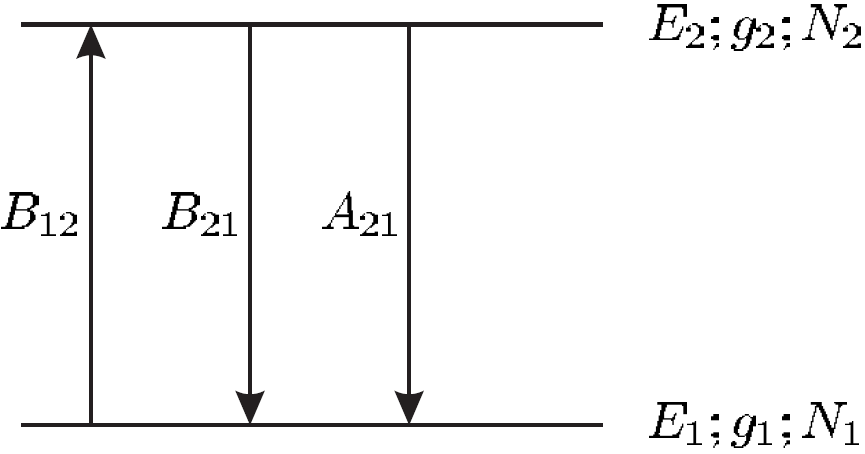
\includegraphics[width=0.5\textwidth]{Q02/images/TwoLevelSystem2.PNG}
    \caption{Toniveausystem med energier $E_1$ og $E_2$, som kan være udarter med $g_1$ og $g_2$, samt har en startpopulation på $N_1$ og $N_2$. Einsteinkoefficienterne $B_{12}$, $B_{21}$ og $A_{21}$ angiver hhv. (stimuleret) absorption, stimuleret emission og spontan emission.}
    \label{fig:Q02_TwoLevelSystem}
\end{figure}

Vi betragter et toniveausystem med energier $E_1$ og $E_2$ i hhv. tilstand $\ket{1}$ og $\ket{2}$. Energiniveauerne har en udartethed (eng. degeneracy) på hhv. $g_1$ og $g_2$, og niveauerne starter med at indeholde hhv. $N_1$ og $N_2$ atomer. Vi sender lys med enrgitæthed $\rho(\omega)$ per frekvensenhed ind på vores toniveausystem, hvilket skaber overgange fra $\ket{1}$ til $\ket{2}$ med en rate, der er proportional med $\rho(\omega_{12})$, hvor proportionalitetskonstanten er $B_{12}$. Atomet interagerer kun med den del af energifordelingen $\rho(\omega)$, som har en frekvens tæt på atomets \textsf{resonansfrekvens} $\omega_{12} = (E_1 - E_2)/\hbar$. Per symmetri vil det også formodes, at lyset vil skabe overgange fra $\ket{2}$ til $\ket{1}$ med en rate, der stadig er proportionel med $\rho(\omega)$, men har proportionalitetskonstant $B_{21}$. Førstnævnte er et tilfælde af (stimuleret) absorption, mens sidstnævnte er et tilfælde af stimuleret emission, hvor lyset med vinkelfrekvens $\omega$ vil få atomet til at udsende lys med denne samme frekvens.\footnote{This increase in the amount of light at the incident frequency is findaental to the operation of lasers. The word \textsf{laser} is an acronym for Light Amplification by Stimulated Emission of Radiation.} Denne symmetri mellem stimuleret absorption og emission bliver dog ødelagt af spontan emission, hvor en elektron falder ned til det laveste energiniveau ($\ket{2} \rightarrow \ket{1}$) selvom den ikke er blevet belyst. Raten af denne spontane emission beskrives ved $A_{21}$.

\underline{Opsummeret:} Bliver et atom ramt af lys med frekvens $\omega$ tæt på atomets resonsfrekvens $\omega_{12} = \Delta E / \hbar$ vil der ske en ændring af populationen i energiniveauerne ved en af følgende muligheder, beskrevet ved de givne Einsteinkoefficienter:
\begin{itemize}
    \item $B_{12}$: \textbf{Absorption} af en foton exciterer en elektron fra $\ket{1}$ til $\ket{2}$.
    \item $B_{21}$: Absorption af en foton vil (per symmetri) udløse en \textbf{stimuleret emission} af en foton af samme frekvens som den indkomne, samt lade en elektron falde fra $\ket{2}$ ned til $\ket{1}$.
    \item $A_{21}$: Uden at blive ramt af de indkomne fotoner kan der forekommer \textbf{spontan emission}, hvilket udsender en foton med atomets resonsnsfrekvens og derved bringe en elektron fra $\ket{2}$ til $\ket{1}$. Dette forekommer med en rate (eng. decay rate) på $A_{21} = 1/\tau$, hvor $\tau^{-1}$ er den gennemsnitlige levetid for $\ket{2}$.
\end{itemize}

Rateligningerne (eng. the rate equations) for populationerne $N_1$ og $N_2$ for tilstandene $\ket{1}$ og $\ket{2}$ bliver derved
\begin{align}
    \frac{\text{d}N_2}{\text{d}t} &= N_1 B_{12} \rho(\omega_{12}) - N_2 B_{21} \rho(\omega_{12}) - N_2 A_{21} \: , \quad \text{og} \label{eq:Q02_RateEquationN2}\\
    \frac{\text{d}N_1}{\text{d}t} &= - \frac{\text{d}N_2}{\text{d}t} \: , \label{eq:Q02_RateEquationN1} \: .
\end{align}
\Cref{eq:Q02_RateEquationN2} giver ændringsraten for $N_2$ som funktion af hhv. absorption, stimuleret emission og spontal emission, mens \cref{eq:Q02_RateEquationN1} er en konsekvens af, at der kun er to energiniveauer, så elektronerne, som forlader $\ket{2}$, må komme til $\ket{1}$.

Idet at der intet lys er ($\rho(\omega) = 0$), og der befinder sig elektroner i $\ket{2}$ ($N_2(0) \ne 0$), så vil ligningerne få en eksponentielt aftagende løsning
\begin{align}
    N_2(t) &= N_2(0)\exp{-A_{21}t} = N_2(0)\exp{-\frac{t}{\tau}} \: ,
\end{align}
hvor $\tau$ er den gennemsnitlige levetid.


\paragraph{Sammenhæng mellem A og B koefficienterne:} For at finde sammenhængen mellem Einsteinkoefficienterne betragtes det føromtalte atom (toniveausystem) beliggende i et område af sortlegemestråling (eng. black-body radiation). Her vil energitætheden $\rho(\omega)\,\text{d}\omega$ i vinkelfrekvensintervallet $[\omega,\: \omega + \text{d}\omega]$ kun afhænge af temperaturen $T$ af sortlegemet. Dette er givet af Plancks lov
\begin{align} \label{eq:Q02_PlancksLov}
    \rho(\omega) &= \frac{\hbar\omega}{\pi^2c^3} \dfrac{1}{\exp{\dfrac{\hbar\omega}{k_B T}} - 1} \: .
\end{align}
Betragtes nu på populationerne, når der er ligevægt (eng. equilibrium), $\frac{\text{d}N_2}{\text{d}t} = 0$, så populationerne ikke ændrer sig, så kan 
\begin{align} \label{eq:Q02_rho(omega)ILigevaegt}
    0 &= N_1 B_{12} \rho(\omega_{12}) - N_2 B_{21} \rho(\omega_{12}) - N_2 A_{21} \nonumber\\
    N_2 A_{21} &= \left(N_1 B_{12} - N_2 B_{21}\right) \rho(\omega_{12}) \nonumber\\
    \Rightarrow \rho(\omega_{12}) &= \frac{A_{21}}{B_{21}} \dfrac{1}{\dfrac{N_1 B_{12}}{N_2 N_{21}} - 1} \: .
\end{align}
I termisk ligevægt vides det, at populationerne i hvert af tilstandene\footnote{Der er $g_i$ udartede tilstande i ét energiniveau $E_i$}, som er i energiniveauerne, vil være givet ved Boltzmannfaktoren, og populationen i hver af tilstandene er giver som populationen i energiniveauet delt med antallet af udartede tilstande i niveauet, hvorfor
\begin{align} \label{eq:Q02_VedBrugAfTermiskLigevaetOgBoltzmannfaktoren}
    \frac{N_2}{g_2} &= \frac{N_1}{g_1}\exp{-\frac{\hbar\omega}{k_B T}} \: .
\end{align}

Kombineres \cref{eq:Q02_PlancksLov,eq:Q02_rho(omega)ILigevaegt,eq:Q02_VedBrugAfTermiskLigevaetOgBoltzmannfaktoren} fås
\begin{align}
    A_{21} & =\frac{\hbar\omega^3}{\pi^2c^3} B_{21} \: , \quad \text{og} \label{eq:Q02_A21} \\
    B_{12} &= \frac{g_2}{g_1} B_{21} \: , \label{eq:Q02_B12SomFunktionAfB21}
\end{align}
hvilket er relationen mellem Einsteinkoefficienterne, som er egenskaber ved atomet, hvorfor forskellige atomer vil have forskellige koefficienter, men de gør sig gældende for enhver type lys. Det er vigtigt at notere, at stærk absorption associeres med stærk emission, hvilket kan ses af \cref{eq:Q02_A21}.


\paragraph{Relation af Einsteinkoefficienterne til spektroskopiske eksperimenter:} \ldots